\documentclass{standalone}
\usepackage{tikz}
\usepackage{tikz-feynman}

\begin{document}
%% \feynmandiagram [spring layout, vertical=w1 to b] {
%%   h1 [particle=$H$] -- [charged scalar] b [blob] -- [fermion, edge label'=$\bar{d}$] y1 -- [anti fermion, edge label'=$Q$] w1 -- [anti fermion, edge label'=$Q$] y2 -- [fermion, edge label'=$\bar{u}^\dagger$] b,
%%   l0 [particle=$L$] -- [fermion] w2 -- [fermion, edge label'=$L$] y3 -- [anti fermion, edge label'=$\bar{e}^\dagger$] b,
%%   h3 [particle=$H$] -- [charged scalar] y2,
%%   h2 [particle=$H$] -- [charged scalar] y1,
%%   %% h2 -- [opacity=0] h3,
%%   w1 -- [edge label'=$W$, photon] w2,
%%   h2 -- [opacity=0] y3,
%%   %% d [particle=$\bar{d}$] -- [fermion] b,
%%   %% h2 [particle=$H$] -- [charged scalar] y1,
%%   %% h1 [particle=$H$] -- [charged scalar] y2 -- q
%%   %% u [particle=$\bar{u}^\dagger$] -- [anti fermion] y1 -- ,
%%   h4 [particle=$H^\dagger$] -- [anti charged scalar] y3,
%%   l2 [particle=$L$] -- [fermion] b,
%% };
%%
%% \feynmandiagram [layered layout, vertical=l to h] {
%%   l [particle=$L$] -- [fermion] b [blob],
%%   h [particle=$H$] -- [charged scalar] b,
%%   b -- [fermion, edge label'=$\bar{d}$, out=90, in=180] d --
%%   [anti fermion, out=0, in=90, edge label'=$Q$] g1,
%%   b -- [anti fermion, out=0, in=180, edge label'=$\bar{u}^\dagger$] u,
%%   u -- [opacity=0] g2,
%%   u -- [fermion] g1,
%%   b -- [opacity=0] h2,
%%   b -- [anti fermion, edge label'=$\bar{e}^\dagger$, out=270, in=180] e -- [anti fermion, in=270, out=0, edge label'=$L$] g2,
%%   {[same layer] g2 -- [photon, edge label=$W$] g1},
%%   {[same layer] d -- [opacity=0] u},
%%   {[same layer] u -- [opacity=0] e},
%%   {[same layer] u -- [charged scalar] h2},
%% };

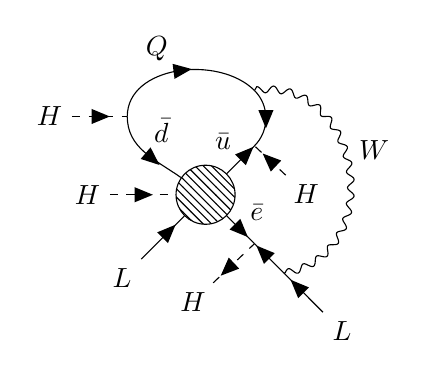
\begin{tikzpicture}
  \begin{feynman}
    \node [blob] (b);
    \vertex [left=of b] (hl) {$H$};
    \vertex [below left=of b] (ll) {$L$};
    \vertex [above left=4em of b] (yd);
    \vertex [below right=2.5em of b] (ye);
    \vertex [above right=2.5em of b] (yu);
    \vertex [below left=2em of ye] (he) {$H$};
    \vertex [below right=1.5em of ye] (ge);
    \vertex [below right=2em of ge] (rl) {$L$};
    \vertex [left=2em of yd] (hd) {$H$};
    \vertex [below right=1.5em of yu] (hu) {$H$};
    \vertex [above=2em of yu] (gq);

    \diagram* {
      (hl) -- [charged scalar] (b) -- [anti fermion] (ll),
      (b) -- [fermion, edge label=$\bar{e}$] (ye) -- [anti fermion] (ge) -- [anti fermion] (rl),
      (he) -- [anti charged scalar] (ye),
      (b) -- [out=145, in=270, anti fermion, edge label'=$\bar{d}$] (yd) -- [out=90, in=135, fermion, edge label=$Q$] (gq) -- [out=315, in=45, fermion] (yu) -- [anti fermion, edge label'=$\bar{u}$] (b),
      (hd) -- [charged scalar] (yd),
      (hu) -- [charged scalar] (yu),
      (ge) -- [photon, half right, edge label'=$W$] (gq),
    };

  \end{feynman}
\end{tikzpicture}

\end{document}
